%!TEX root = ../template.tex
%%%%%%%%%%%%%%%%%%%%%%%%%%%%%%%%%%%%%%%%%%%%%%%%%%%%%%%%%%%%%%%%%%%%
%% chapter2.tex
%% NOVA thesis document file
%%
%% Chapter with the template manual
%%%%%%%%%%%%%%%%%%%%%%%%%%%%%%%%%%%%%%%%%%%%%%%%%%%%%%%%%%%%%%%%%%%%
\chapter{Estado del Arte}
\label{cha:users_manual}

% ================
% = Introduction =
% ================

%%\section{Introduction} % (fold)
%%\label{sec:introduction}
%%
%%{\LARGE \textbf{~\\These instructions are outdated! Please see also the “template.tex” file!\\}}

%%This chapter describes how to use the \LaTeX\ \novathesis\ template (and the “\novathesisclass” class file).

%%Let's start with some simple suggestions:

%%\begin{enumerate}
%%  \item No! You don't have to use this template to write your thesis.  You don't even have to use \LaTeX.  However, writing a thesis is serious stuff, and which tool you shall use to write it is not a decision to make lighthearted.
%%  \item \LaTeX\ is hard enough by itself.  This template aims at making your life easier, but not easy. If you choose to use this template to write your thesis, you are very welcome.  However, don't expect me to provide you help with \LaTeX.  Look for help with your friends (you have some friends, don't you?), or search the web, or try even to read some book(s) on \LaTeX. In the end you will certainly find the experience rewarding.
 %% \item So, don't forget, when you come to the point of “\emph{How do I do this with \LaTeX?}” look for help!  Google is your best friend. 
%%  \item If you believe the difficulty is related with the \novathesis\ template itself (and not with \LaTeX), please \textbf{do not} send me an email asking for help.  Please look for help in the \novathesis\ Google Group (URL) and the \novathesis\ Facebook group (URL).  If you can't find help there from previous posts/messages, then post your own question. Hopefully someone will answer you.
%%\end{enumerate}

%%Now, let's go to a major issue for Windows users.  Characters have to be encoded in files as numbers, and that is how character encodings were born. ASCII and EBCDIC standards are long lost in the past.  The world now uses UTF-8.  Well, not all the world… Windows is still stick in its \emph{codepages}, and “latin1” is what windows uses as the codepage for Western Europe. This messes up with the template. Please be sure you use an editor with UTF-8 support.  \emph{Go to the preferences/options/… of your text editor and set up its default file encoding as UTF-8.}

% section introduction (end)

% ====================
% = Folder Structure =
% ====================
\section{Marco de Referencia Teórico} % (fold)
\label{sec:Marco de Referencia Teórico}

\subsection{Conceptos Generales de una SD-WAN}
\label{sec:Conceptos Generales de una SD-WAN}
SD-WAN es una aplicación específica de la tecnología de redes SDN aplicada a las conexiones WAN utilizadas para conectar redes empresariales sobre grandes distancias geográficas suministrando una arquitectura "Overlay" moviendo el plano de control a la nube, sea esta pública o privada. Según SDN central, puede definirse como un enfoque de software centrico a las tecnologías de "Networking" que reducen los costos operacionales y de capital ("Capex y Opex") mediante un control programático de la infraestructura de red, facilitando la optimización e innovación.
\\
\subsection{Modelos de Programabilidad de Red}
\label{sec:Modelos de Programabilidad de Red}

Existen actualmente 4 modelos de programabilidad de red, considerados como arquitecturas SDN, la diferenciación fundamental entre los 4 modelos consiste en la forma como el plano de control se comunica con el plano de datos de los dispositivos, estos modelos pueden resumirse como sigue:
\begin{itemize}
\item[•] \textbf{APIs programables:}  la primera aproximación a SDN es la inclusión de API dentro de los dispositivos de red, en este modelo sin embargo no hay un desacoplamiento de los planos de datos y control y estos siguen estando dentro, los equipos de red se comunican directamente con las aplicaciones a través de APIs u otro mecanismo como NETCONF. \textbf{Ver figura 5.1(a) Apis Programables}.

\item[•] \textbf{SDN Clásico}: En este modelo el plano de control y el plano de datos si se encuentran desacoplados completamente, el plano de control se comunica con las aplicaciones mediante APIs y con el plano de datos mediante Openflow u otro protocolo propietario Ver \textbf{Ver figura 5.1(b) SDN Clásico}.

\item[•] \textbf{SDN Híbrido:} funciona bajo el mismo concepto que la arquitectura clásica de SDN, con la diferencia de que en este caso los dispositivos mantienen su propio plano de control pero siguen comunicándose con las aplicaciones a través de Openflow mediante una controladora que mantiene el plano de control de todos los equipos. \textbf{Ver figura 5.1(c) SDN Híbrido}.

\item[•]\textbf{Virtualización de Red:} la tendencia de la virtualización ha dividido las redes en un dominio físico y uno virtual, la tendencia es que las decisiones de enrutamiento y seguridad se hagan por software en el plano de virtualización, la comunicación entre este plano virtual y el físico se realiza mediante tecnologías desarrolladas por los fabricantes de software de virtualización, uno de los ejemplos más conocidos es NFX. \textbf{Ver figura 5.1(d) Virtualización de Red}.

\begin{figure}[htbp]
  \centering
  \subcaptionbox{Apis Programables\label{fig:leftsubfig}}%
    {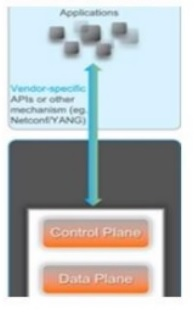
\includegraphics[width=0.2\linewidth]{figure7}}%
  \subcaptionbox{SDN Clásica\label{fig:rightsubfig}}
    {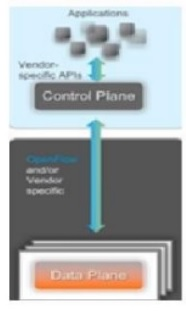
\includegraphics[width=0.2\linewidth]{figure8}}%
  \subcaptionbox{SDN Híbrida\label{fig:rightsubfig}}
    {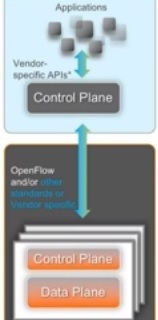
\includegraphics[width=0.2\linewidth]{figure9}}%
  \subcaptionbox{Virtualización de Red\label{fig:rightsubfig}}
    {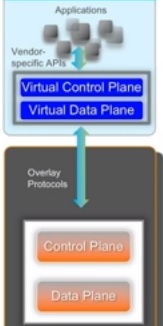
\includegraphics[width=0.2\linewidth]{figure10}}%
  \caption{Modelos Programables de Red}
  \label{fig:fig2subfig}
\end{figure}

\end{itemize}
\subsection{NFV}
\label{sec:NFV}

Network Function Virtualization o NFV ofrece una nueva forma de diseñar, aprovisionar y administrar los servicios de red, desacoplando las funciones de red de los hardware propietarios y realizando funciones en software como NAT, firewall y DNS por nombrar algunos ejemplos. Esta tecnología se encuentra diseñada para consolidar los componentes de red requeridos para lograr una infraestructura completamente virtualizada.
Bajo este concepto toda la orquestración y control de los dispositivos físicos se realizaría desde un punto central desde donde se administrarían las funciones de red, desacoplando así las funciones de red de los dospositivos físicos. La siguiente imagen muestra un ejemplo de cómo funcionaría una red bajo este esquema.


\subsection{OpenFlow}
\label{sec:OpenFlow}

Es un protocolo utilizado para suministrar una interfaz abierta para controlar la conectividad y los flujos de dicha conectividad dentro de una red SDN, es un protocolo extensible por lo que permite a los programadores definir elementos adicionales que permitan al protocolo adaptarse a diferentes redes y a nuevas tecnologías. https://www.opennetworking.org/technical-communities/areas/specification/open-datapath/
Openflow funciona principalmente a través de programas Datapath en donde se define el comportamiento esperado para cada tipo de paquete y el camino que debe tomar dentro de la red, para esto openflow utiliza diversos componentes durante su ejecución que pueden verse en la figura xx.(OFN SDN evolution ver 1.0,Open Networking Foundation, 2016.

Cada uno de estos programas de datapath es posteriormente compilado para ser ejecutado en el código nativo de cada uno de los vendedores de los dispositivos de hardware, de esta manera el programa de datapath puede ser utilizado independientemente del vendedor del hardware.


\subsection{NETCONF}
\label{sec:NETCONF}

El protocolo se encuentra definido por el estándar RFC6241 de la IETF y suministra mecanismos para instalar, manipular y eliminar configuración en dispositivos de red utilizando el formato XML.
NETCONF define un mecanismo simple mediante el cual un dispositivo obtiene una API, esto con el objetivo de que las aplicaciones utilicen dicha API para enviar y recibir configuraciones desde y hacia los dispositivos de red, esto utilizando el paradigma RPC de forma que el cliente codifique un RPC en formato XML y lo envíe a un servidor, quien responderá con otro XML codificado.

Conceptualmente el protocolo NETCONF se divide en 4 capas como lo muestra la siguiente imagen:


1.La capa de transporte seguro suministra un camino de comunicación entre cliente y servidor, en general netconf puede ser utilizado sobre cualquier protocolo de transporte que cumpla con ciertas características.
2.La capa de mensajes provee un mecanismo de entramado independiente del transporte para la codificación de RPC y notificaciones.
3.La capa de operaciones define un set de operaciones básicas de protocolos invocados como métodos RPC con parámetros en codificación XML.

\subsection{Modelos de datos}
\label{sec:Modelos de datos}

\subsubsection{YANG}
\label{sec:YANG}


Es un lenguaje de modelado de datos que se utiliza para modelar datos de estado y configuración del protocolo NETCONF y se encuentra definido bajo el RFC 6020 de la IETF, YANG modela la organización jerárquica de los datos como un árbol y provee una descripción clara de cada nodo así como su relación con otros nodos.
YANG define cuatro tipos de nodo para el modelado de datos:

\begin{itemize}
\item[•] Nodo leaf: Contiene datos simples como enteros o strings, contiene un tipo de valor particular y no tiene nodos hijos.
\item[•]Nodo leaf-list: es una secuencia de nodos leaf, en donde cada uno tiene su valor particular.
\item[•]Nodo contenedor: Es utilizado para agrupar nodos relacionados en un sub arbol, este tipo de nodos no tiene valor y sólo tiene nodos hijos. Un contenedor puede contener nodos de cualquier tipo, incluyendo leaf, list, leaf-list o incluso otros contenedores.
\item[•]Nodo lista: Define una secuencia de entradas de lista identificados por el valor de su leaf “key” una lista puede contener varias de estas llaves y contener cualquier número de nodos de cualquier tipo.

\end{itemize}

YANG permite la definición de RPC de NETCONF, los nombres y parámetros de entrada y salida de las operaciones se encuentran modelados utilizando YANG así como las notificaciones. El siguiente ejemplo muestra como se encuentra estructurado un RPC en YANG.


\subsection{RESTful APIs}
\label{sec:RESTful APIs}

Restconf es un protocolo basado en HTTP que suministra una interfaz programática para acceder a datos definidos en YANG utilizando los conceptos de datastore definidos en el protocolo NETCONF.
NETCONF y RESTCONF suelen trabajar en conjunto permitiendo la ejecución de operaciones CRUD, hay dispositivos que soportan los dos protocolos  en conjunto de la siguiente manera:

Al estar basado en HTTP las operaciones CRUD de RESTCONF se realizan mediante los métodos tradicionales, como los son los siguientes:
GET:
POST:
PUSH:
PATCH:
DELETE:

RESTCONF requiere de HTTP para su transporte y requiere soporte de TLS para su transporte, aunque no se especifica que versión específica se requiere para RESTCONF si se recomienda por lo menos HTTP1.1, dado que los servidores RESTCONF deben soportar HTTPS, dichos servidores tienen que presentar un certificado dígital X509v3.

\subsection{RESTCONF}
\label{sec:RESTCONF}

RESTCONF requiere de HTTP para su transporte y requiere soporte de TLS para su transporte, aunque no se especifica que versión específica se requiere para RESTCONF si se recomienda por lo menos HTTP1.1, dado que los servidores RESTCONF deben soportar HTTPS, dichos servidores tienen que presentar un certificado dígital X509v3.

\subsection{Marco de referencia tecnológico}
\label{sec:Marco de referencia tecnológico}

La solución definida en este proyecto es el IWAN de Cisco, en el capitulo “selección de la solución” en este mismo documento se plantean las razones por las cuales se seleccionó IWAN como la mejor solución para el caso de este cliente. Por tanto este apartado estará dedicado a las tecnologías que componen la solución de IWAN.


\subsection{IWAN}
\label{sec:IWAN}

IWAN es una solución SD-WAN propietaria de Cisco cuyo objetivo es la reducción de costos para el transporte de la información del cliente al hacer viable mediante una serie de tecnologías la utilización de enlaces menos costosos como internet, en esta solución el tráfico se enruta de manera dinámica según las condiciones de la aplicación, la solución está diseñada para empresas cuyas sucursales tengan un aumento en su tráfico WAN por el uso de aplicaciones en la nube, Cisco dice ofrecer las siguientes ventajas con su aplicación de IWAN:



IWAN se compone de varias tecnologías que hacen de la solución una alternativa efectiva para las sucursales que utilizan tanto consumo de aplicaciones centralizadas como aplicaciones en la nube:


\begin{itemize}
\item[•]Independencia de transporte: La solución utiliza DMVPN para la creación de túneles dinámicos entre todas las sedes, estos túneles se encuentran encriptados para garantizar un componente de seguridad sobre el transporte aunque vaya por la red pública, esto permite obtener una topología full-mesh de manera automática y al mismo tiempo obtener una configuración independiente del tipo de transporte y del proveedor de servicios que sea contratado.
\item[•]Enrutamiento basado en aplicación: La solución utiliza además de EIGRP como protocolo de enrutamiento, una solución propietaria de Cisco llamada performance routing, que permite tomar decisiones de enrutamiento basándose en el estado actual de los enlaces y en las necesidades de calidad de servicio de cada aplicación.
\item[•]Gestión centralizada: mediante la controladora SDN APIC-EM es posible gestionar los equipos remotos desde un punto centralizado y realizar cambios a una gran cantidad de dispositivos al mismo tiempo, agilizando y automatizando los cambios de red.
\item[•]Optimización de recursos WAN: la solución incluye una tecnología de compresión de tráfico llamada WAAS que permite ahorrar costos en los enlaces WAN haciendo más efectivo el uso del ancho de banda.

La controladora SDN que utiliza esta tecnología se denomina APIC-EM, esta controladora no solamente cumple la función de plano de control sino que también contiene aplicaciones de red embebidas que aprovechan la naturaleza centralizada de la controladora, entre esas aplicaciones se encuentra IWAN, que es la solución SD-WAN puntual que se presenta en este documento, la controladora SDN sin embargo es el puente entre la aplicación y la red física, esto puede apreciarse con mayor detalle en la siguiente imagen:


Una de las mayores ventajas de esta controladora es que no necesita de equipos de red especiales que soporten los protocolos de SDN, aunque esto último es lo recomendado el APIC-EM trae las ventajas de SDN sin requerir de una gran inversión en cambio de equipos de red, lo que lo hace una opción bastante atractiva para una compañía que quiera empezar a adentrarse en la programabilidad de la red sin requerir una inversión inicial tan fuerte.
\end{itemize}

\subsection{DMVPN}
\label{sec:DMVPN}

DMVPN(Dynamic Multipoint VPN) es la solución de transporte propietaria de Cisco que hace parte de la solución de IWAN, es una solución de overlay en donde las ubicaciones remotas establecen un túnel estático hacia una ubicación central(hub) y establece túneles de manera dinámica entre diferentes ubicaciones remotas(spokes). Esto permite tener conectividad full-mesh sin tener que realizar las configuraciones de todos los túneles de forma manual, los túneles entre spokes son removidos después de un periodo de inactividad, liberando así recursos de memoria y CPU y por tanto eliminando la necesidad de routers tan robustos en las sedes remotas, los equipos de enrutamiento de mayor capacidad deben ser por tanto utilizados en el sitio central (hub). La siguiente imagen muestra el comportamiento dinámico de DMVPN.
\\
DMVPN utiliza diversas tecnologías para lograr este objetivo, las más relevantes se enuncian a continuación.


\begin{itemize}
\item[•]túneles mGRE: mGRE es un protocolo de entunelamiento capaz de transportar múltiples protocolos como IPv4, IPv6 y otros, estos túneles son asignados a una interface física y requieren direccionamiento propio en la interfaz del túnel, la diferencia entre esta tecnología y los túneles GRE tradicionales es que mGRE puede conectar más de 2 dispositivos utilizando el mismo túnel.  
los túneles se forman agregando un encabezado IP externo al paquete con la información IP fuente y destino correspondiente a las interfaces fuente y destino del túnel como lo muestra la figura x.
\item[•]NHRP:  Este protocolo se encuentra definido bajo el RFC 2332, y es utilizado para que un equipo fuente determine el siguiente salto hacia un destino en una red NBMA, es decir realiza una resolución de direccionamiento, similar a lo que ocurre con ARP en la resolución de dirección IP a direccion MAC. El protocolo funciona utilizando un NHS que se encarga de la resolución de direccionamiento dentro de la nube de NHRP, por su parte los equipos NHC son aquellos que realizan las peticiones de NHRP hacia el NHS.
La siguiente imagen representa el funcionamiento de NHRP en terminos generales:
\item[•]Adicional al registro de los NHC con los NHS, NHRP tiene la capacidad de que los NHC encuentren un camino más corto sobre la infraestructura o formar uno mediante una conexión virtual directamente hacia otro NHC, esta habilidad es utilizada en DMVPN para establecer una topología full mesh sin todo el trabajo administrativo que esto conlleva.
\end{itemize}

\subsection{WAAS}
\label{sec:WAAS}

Por su parte WAAS es una tecnología propietaria de Cisco que se encarga de optimizar el tráfico TCP en la red con el principal objetivo de disminuir la utilización de ancho de banda utilizando algoritmos de compresión para este fin. Son varias las tecnologías que reúne WAAS para la optimización del ancho de banda a nivel WAN, de ellas vale la pena resaltar las 3 más relevantes.

\begin{itemize}
\item[•]TFO Optimization: utiliza varias tecnologías de optimización de flujo para optimizar el tráfico TCP, realizando funciones como escalamiento de ventanas TCP, maximización del tamaño de ventana inicial, Buffering incrementado, BIC TCP.
\item[•]Compresión: utiliza algoritmos de eliminación de datos redundantes (DRE) y compresión LZ para optimizar el tráfico WAN.
\item[•]Aceleración específica de aplicaciones: analiza y predice el tráfico de una aplicación para transformar una secuencia de comandos en una más pequeña, generando así ahorro en la utilización del ancho de banda.
\end{itemize}


\subsection{EIGRP}
\label{sec:EIGRP}


EIGRP es el protocolo seleccionado por Cisco para hacerse cargo del plano de enrutamiento en la solución SD-WAN, este protocolo aunque Cisco lo considera como un protocolo híbrido con características de protocolos vector distancia y de protocolos estado de enlace, es realmente un protocolo vector distancia ya que no mantiene la topología general del sistema autónomo. Sin embargo este ha demostrado ser un protocolo escalable y de convergencia rápida por lo que se integra adecuadamente en el diseño de IWAN.
EIGRP logra una convergencia rápida mediante la construcción de una tabla topológica utilizando la información enseñada por sus vecinos, la diferencia entre esta tabla topológica y la construida por un protocolo de estado de enlace es que  EIGRP al ser un protocolo vector distancia solo le enseña a sus vecinos las mejores rutas y no todas las rutas que conoce como sería el caso en un protocolo estado de enlace. Aún así la convergencia es extremadamente rápida ya que basado en su métrica el protocolo selecciona la mejor ruta (succesor) y la segunda mejor ruta (feasable succesor), de esta forma cuando una red deja de aprenderse por la mejor ruta el protocolo utiliza inmediatamente la segunda mejor ruta, por tanto obteniendo unos tiempos de milisegundos para la convergencia.
Para distribuir las rutas a través de la red EIGRP utiliza actualizaciones de enrutamiento incrementales y no periódicas, esto quiere decir que solo se envía un update cada vez que hay un cambio en la red. EIGRP depende por lo tanto de sus relaciones de vecinos para propagar de manera confiable los cambios en la tabla de enrutamiento a través de la red. Esta relación de vecindad se forma cuando dos routers corriendo EIGRP ven los paquetes Hello del otro equipo, estos paquetes son enviados cada 5 segundos.
EIGRP utiliza una métrica compuesta por los siguientes parámetros para calcular la ruta más corta:

\subsection{PfR}
\label{sec:PfR}

PfR es parte integral de la solución de IWAN, y es la mayor responsable de la inteligencia de la solución, su objetivo es mejorar el rendimiento y disponibilidad de las aplicaciones realizando una optimización del control de enrutamiento basándose en los requerimientos de cada aplicación. PfR monitorea el rendimiento de red y selecciona el mejor camino basándose en criterios de alcanzabilidad, delay, jitter y pérdida de paquetes mientras balancea el tráfico entre los enlaces disponibles.
PfR define varios roles para los dispositivos que componen la solución, dichos roles son master controler (MC) y border router (BR), el MC actúa como plano de control para el PfR y el BR sería el plano de datos al seleccionar el camino basándose en las decisiones tomadas por el MC.
En PfR las políticas de tráfico son definidos basados en DSCP o en la aplicación por sí misma, que se identifica mediante AVC (Application visibility and Control). dichas políticas contienen la información de requerimientos en cuanto a parámetros de retardo, jitter y pérdida de paquetes para cada aplicación así como la preferencia de camino de cada una de ellas. Una vez definida la política PfR detecta el tráfico y comienza a realizar mediciones de ancho de banda y rendimiento, posteriormente el MC toma la decisión mediante la comparación de métricas en tiempo real y le da la instrucción al BR de utilizar el camino apropiado. La imagen X muestra el flujo de la operación de PfR:


Dentro de los roles de MC y BR existen dos variantes, los equipos Hub y los Branch, los equipos Hub son los responsables del plano de control en el caso del MC y del plano de datos en el caso del BR para toda la topología de red, el HUB MC se encarga mediante SAF de propagar las políticas, especificaciones de los monitores para medir rendimiento de los canales y prefijos de los sitios a los MC en cada Branch y a los HUB BR, los BRANCH MC a su vez propagan las políticas a los BRANCH BR. La siguiente imagen detalla este flujo de información entre los elementos de IWAN. 

\newpage

\noindent
\begin{tabularx}{\linewidth}{>{\ttfamily}l>{\itshape}l>{\upshape}X}
novathesis.cls     & file    & 
The main class file. It will include additional files from \texttt{novathesis-files} folder. 


\\ 
template.tex      & file    & 
The main user file. Use this file as the main file for your thesis. 
\\
bibliography.bib  & file    & 
An example of a bibliography file. You may have has many as you want. \\
template.pdf      & file    & 
A possible result of applying pdf\LaTeX\ to the \texttt{template.tex} file. The template supports multiple types of documents (e.g., MSc dissertation, PhD thesis, …) and multiple Schools (e.g., FCT-NOVA, FCSH-NOVA, IST-UL, FC-UL, …) and each will produce different results.
\\
Chapters          & folder  & Examples of thesis chapters. Replace them with your own chapters. 
\\
Examples          & folder  & Some more examples of the use of the template for different document types and Schools. 
\\
Scripts           & folder  & Some (possibly useful) scripts for Unix-based systems (Linux, Mac OSx). If you are a windows user, ignore this folder (you may safely delete it if you want). 
\\
novathesis-files   & folder  & 
Additional files for the \novathesisclass\ file.  Unless you know what you are doing, avoid messing up with the files and folders inside this folder (except for deleting the unused Schools, see below). 
\\
\end{tabularx}

The \texttt{novathesis-files} folder contains additional files and folders that complement the main \novathesisclass\ file.  These are:

\noindent
\begin{tabularx}{\linewidth}{>{\ttfamily}l>{\itshape}l>{\upshape}X}
README.txt      & file    &
A file that should be read!  :) 
\\
fix-babel.clo   & file    &
Simple fixes to the \texttt{babel} package.
\\
lang-text.clo   & file    &
Translations of important strings used in the template.  Currently fully supported are Portuguese and English, but French is on the way.  If you add translations for your own language, please be so kind and send them to me. Thank you!
\\
options.clo     & file    &
Processing of \novathesisclass\ options.  \emph{Don't mess with this!}
\\
packages.clo    & file    &
Additional packages to be loaded into the \novathesis\ template. \emph{You should not mess with this!}
\\
spine.clo       & file    &
This file is loaded only if the option \texttt{spine=true}, and includes the typesetting of the book spine.
\\
ChapStyles      & folder  &
Contains a lot of files, one for each chapter style.  If you really know what you are doing, you may add your own chapter style here.
\\
FontStyles      & folder  &
Contains a few files, one for each set of fonts (main text font, chapter font, section font, subsection font, etc).  If you really know what you are doing, you may add your own set here.
\\
Schools         & folder  &
Configuration files for each school.  This folder is organized into subfolders, one for each university.  \emph{You may safely delete all the subfolders except the one for your University.}  Then open the subfolder of your University and \emph{you may safely delete all the subfolders except the one for your School/Faculty}.
\\
\end{tabularx}

As stated above, the \texttt{Schools} folder contains per-university folders and per-school (faculty) subfolders.  Currently these are the available folders:

\noindent
\begin{tabularx}{\linewidth}{>{\ttfamily}r@{~/~}>{\ttfamily}l>{\itshape}l>{\upshape}X}
ul     & ist    & folder  & 
The folder for the \href{http://www.tecnico.ulisboa.pt}{\emph{Instituto Superior Técnico}} of the \emph{University of Lisbon}.
\\
nova    & fcsh   & folder  & 
The folder for the \href{http:www.fcsh.unl.pt}{\emph{Faculty of Human and Social Sciences}}  of the \emph{NOVA University of Lisbon}.
\\
nova    & fct    & folder  & 
The folder for the \href{http:www.fct.unl.pt}{\emph{Faculty of Sciences and Technology}} of the \emph{NOVA University of Lisbon}.
\\
nova    & novaims    & folder  & 
The folder for the \href{http:www.novaims.unl.pt}{\emph{Information and Management School}} of the \emph{NOVA University of Lisbon}.
\\
\end{tabularx}

% section folder_structure (end)

% ===================
% = Package options =
% ===================
\section{\novathesisclass\ Class Options} % (fold)
\label{sec:package_options}

The \novathesis\ class can be customized with the options listed below.

\newcommand{\classoption}[3]{\textbf{#1=OPT}\qquad #2\\\qquad\emph{#3}\\}

\noindent
\begin{ctabular}{@{}p{\linewidth}@{}}
  \toprule
  \classoption{docdegree}%
    {phd(*), phdplan, phdprop, msc, mscplan, bsc}%
    {The type of the document: PhD Thesis (default), PhD Plan, PhD Proposal, MSc Disseration, MSc Plan, BSc Report}
    \midrule
  \classoption{school}%
		{nova/fct(*), nova/fcsh, nova/ims, ul/ist, ul/fc}%
    {The name of the school. This option changes the typesetting of the cover and some School specific formating, like margins, fonts, paragraph spacing and indentation, etc…}
    \midrule
  \classoption{lang}%
    {en(*), pt}%
    {The main language for the document.  Currently only Portuguese and English are supported.  Other languages are expected to be support in forthcoming versions.}
    \midrule
  \classoption{fontstyle}%
    {bookman, charter, fourier, kpfonts(*), mathpazo1, mathpazo2, newcent}%
    {The font set to be used in the document.  Please note that a font set include definitions for the main text, headings, maths, etc.}
    \midrule
  \classoption{chapstyle}%
    {bianchi, bluebox, brotherton, dash, default, elegant(*), ell, ger, hansen, ist, jenor, lyhne, madsen, pedersen, veelo, vz14, vz34, vz43}%
    {The chapter style, i.e., the look of the chapter beginning.}
    \midrule
  \classoption{converlang}%
    {en, pt(*)}%
    {The language to be used when typesetting the cover page.}
    \midrule
  \classoption{otherlistsat}%
    {front(*), back}%
    {Where to put the other lists besides the table of contents. The default is (\texttt{front}) before the main text.  But some scientific areas prefer them at the end of the document (\texttt{back}), just before the Appendixes.}
    \midrule
  \classoption{aftercover}%
    {true, false(*)}%
    {Include or don't include the contents of the “\texttt{aftercover}” file. The default is for this file to be ignored (if if it exists).}
    \midrule
  \classoption{linkscolor}%
    {darkblue(*), black}%
    {The color for all the hyperlinks in the PDF file.  The “\texttt{media=paper}” option (see below) will override this option to “\texttt{black}”}
    \midrule
  \classoption{spine}%
    {true, false(*)}%
    {Generate the book spine and the last page in the PDF.}
    \midrule
  \classoption{biblatex}%
    {OPT=\{list of options for \texttt{biblatex}\}}%
    {Customize \texttt{biblatex}, the bibliography management system used in this class. Probably you will want to change the value of the \texttt{biblatex} “\texttt{style}” option. For other customizations of \texttt{biblatex} check its manual.}
    \midrule
  \classoption{memoir}%
    {OPT=\{list of options for \texttt{memoir}\}}%
    {Customize the base class \texttt{memoir}. The \texttt{memoir} manual should be the first document to be consulted when looking for “\textbf{how can I do this?}” You may wnat to change the base font size from 11pt to a smaller (10pt) or larger (12pt) size.  Also, remember to change the “\texttt{draft}” to final when your document is finished.}
    \midrule
  \classoption{media}%
    {screen(*), paper}%
    {Behavior to be customized in the school options/configuration. Expected definitions for screen are: left and right margins are equal and use colored links. Expected definitions for paper are: left and right margins are different and use black links.}
    \bottomrule
\end{ctabular}

\section{Additional considerations about the class options} % (fold)
\label{sec:additional_considerations}

In this section we will provide some additional considerations about some of the customizations available as class options.

\subsection{The main language} % (fold)
\label{sub:the_main_language}

The choice of the main language with the option “\texttt{lang=OPT}” affects:

\begin{itemize}
	\item \textbf{The order of the summaries.} First is printed the abstract in the main language and then in the foreign language. This means that if your main language for the document in English, you will see first the “abstract” (in English) and then the “resumo” (in Portuguese). If you switch the main language for the document for Portuguese, it will also automatically switch the order of the summaries to “resumo” and then “abstract”.
	\item \textbf{The names for document sectioning.} E.g., ``Chapter'' vs.\ ``Capítulo'', ``Table of Contents'' vs.\ ``Índice'', ``Figure'' vs.\ ``Figura'', etc.
	\item \textbf{The type of documents in the bibliogrpahy.} E.g., ``Technical Report'' vs.\ ``Relatório Técnico'', ``PhD Thesis'' vs.\ ``Tese de Doutoramento'', etc.
\end{itemize} 

No mater which language you chose, you will always have the appropriate hyphenation rules according to the language at that point. You always get Portuguese hyphenation rules in the ``Resumo'', english hyphenation rules in the ``Abstract'', and then the main language hyphenation rules for the rest of the document.

% subsection the_main_language (end).

% section additional_consideration (end)


\subsection{Class of Text} % (fold)
\label{sub:class_of_text}

You must choose the class of text for the document. The available options are:

\begin{enumerate}
	\item \textbf{bsc} --- BSc graduation report.
	\item \textbf{*mscplan} --- Preparation of MSc dissertation. This is a preliminary report graduate students at DI-FCT-NOVA must prepare to conclude the first semester of the two-semesters MSc work. The files specified by \verb!\dedicatoryfile! and \verb!\acknowledgmentsfile! are ignored, even if present, for this class of document.
	\item \textbf{msc} --- MSc dissertation.
	\item \textbf{phdprop} ---  Proposal for a PhD work. The files specified by \verb!\dedicatoryfile! and \verb!\acknowledgmentsfile! are ignored, even if present, for this class of document.
	\item \textbf{prepphd} ---  Preparation of a PhD thesis. This is a preliminary report PhD students at DI-FCT-NOVA must prepare before the end of the third semester of PhD work. The files specified by \verb!\dedicatoryfile! and \verb!\acknowledgmentsfile! are ignored, even if present, for this class of document.
	\item \textbf{phd} --- PhD dissertation.
\end{enumerate}
% subsection class_of_text (end)

% ============
% = Printing =
% ============
\subsection{Printing} % (fold)
\label{sub:printing}

You must choose how your document will be printed. The available options are:
\begin{enumerate}
	\item \textbf{oneside} --- Single side page printing.
	\item \textbf{*twoside} --- Double sided page printing.
\end{enumerate}
% subsection printing (end)

% =============
% = Font Size =
% =============
\subsection{Font Size} % (fold)
\label{ssec:font_size}

You must select the encoding for your text. The available options are:
\begin{enumerate}
	\item \textbf{11pt} --- Eleven (11) points font size.
	\item \textbf{*12pt} --- Twelve (12) points font size. You should really stick to 12pt\ldots
\end{enumerate}
% subsection font_size (end)

% =================
% = Text encoding =
% =================
\subsection{Text Encoding} % (fold)
\label{ssec:text_encoding}

You must choose the font size for your document. The available options are:
\begin{enumerate}
	\item \textbf{latin1} --- Use Latin-1 (\href{http://en.wikipedia.org/wiki/ISO/IEC_8859-1}{ISO 8859-1}) encoding.  Most probably you should use this option if you use Windows;
	\item \textbf{utf8} --- Use \href{http://en.wikipedia.org/wiki/UTF-8}{UTF8} encoding.    Most probably you should use this option if you are not using Windows.
\end{enumerate}
% subsection font_size (end)

% ============
% = Examples =
% ============
\subsection{Examples} % (fold)
\label{ssec:examples}

Let's have a look at a couple of examples:

\begin{itemize}
	\item Preparation of PhD thesis, in portuguese, with 11pt size and to be printed single sided (I wonder why one would do this!)\\
	\verb!\documentclass[prepphd,pt,11pt,oneside,latin1]{thesisdifct-nova}!
	\item MSc dissertation, in english, with 12pt size and to be printed double sided\\
	\verb!\documentclass[msc,en,12pt,twoside,utf8]{thesisdifct-nova}!
\end{itemize}
% subsection examples (end)

\section{How to Write Using \LaTeX} % (fold)
\label{sec:how_to_write_using_latex}

Please have a look at Chapter~\ref{cha:a_short_latex_tutorial_with_examples}, where you may find many examples of \LaTeX constructs, such as Sectioning, inserting Figures and Tables, writing Equations, Theorems and algorithms, exhibit code listings, etc.

% section how_to_write_using_latex (end)



\section{Example glossary, acronyms, and symbols}
%
% \todo[inline]{A a note in a line by itself.}
%
This is the first occurrence of an abbreviation: \gls{abbrev}. And now the second occurrence of the same abbreviation: \gls{abbrev}. And a new acronym with capital letter: \Gls{xpt} and reused \gls{xpt}.  Let's also use a few other acronyms such as \gls{aaa}, \gls{aab}, \gls{aba}, \gls{bbb} and \gls{xpt}.
In geometry, the area enclosed by a circle of radius \gls{r} is $\pi r^2$. Here the Greek letter \gls{pi} is equal to the ratio of the circumference of any circle to its diameter.
Lets add ``\gls{computer}'' to the glossary!
%
% Please note that
% \begin{center}
%   \textbf{\large this package and template are not official for FCT/NOVA}.
% \end{center}
